\subsection{ماشین مجازی}
همان طور که در قسمت مقدمه گفته شد باید کاربری در
\lr{MySQL}
بسازیم که از تمامی
\lr{IP}ها
اجازه‌ی دسترسی داشته باشد که بتوان از سمت
\lr{host}، \lr{HammerDB}
را بر روی دیتابیس اعمال کرد. بعد از ساخت کابر مانند شکل
\ref{fig:mysql:init:host_to_vm}
کانکشن را تست می‌کنیم.

سپس بر روی کرنل 5
\lr{schema}
را می‌سازیم و آنرا به کمک دستورات قسمت
\lr{bare metal}
مورد بررسی قرار می‌دهیم.
\begin{figure}[H]
    \centering
    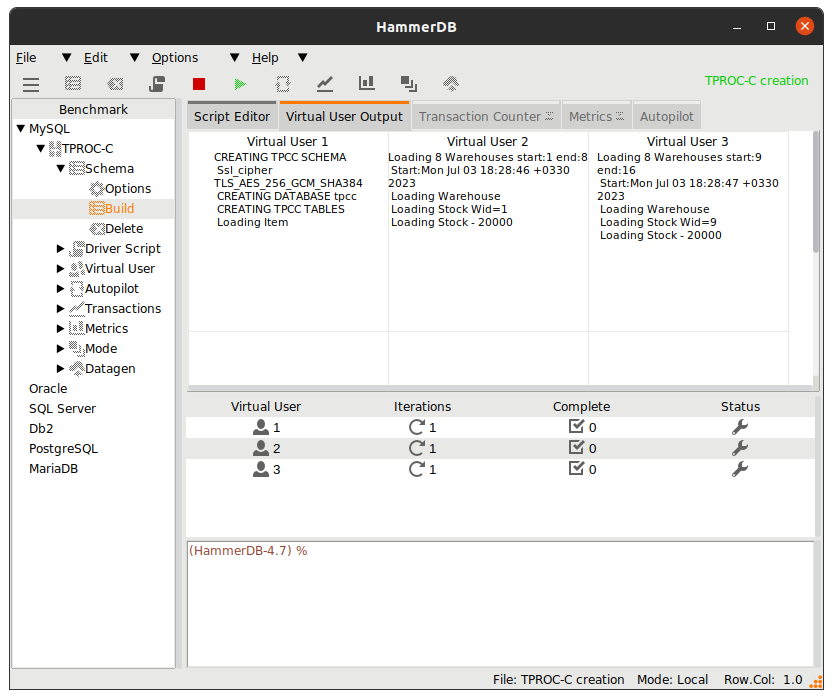
\includegraphics[scale=0.5]{pictures/mysql/vm/schema.png}
    \caption{\lr{schema build} در \lr{VM}}
    \label{fig:mysql:vm:schema}
\end{figure}
اما یک اتفاق خیلی عجیبی که افتاد این بود که در ابتدا مانند قسمت قبل
\lr{TPM}
بعد از مدتی افت کرد ولی دوباره بعد از مدتی بالا رفت! به شکل
\ref{fig:mysql:vm:tpm}
توجه کنید.
\begin{figure}[H]
    \centering
    \subfloat{{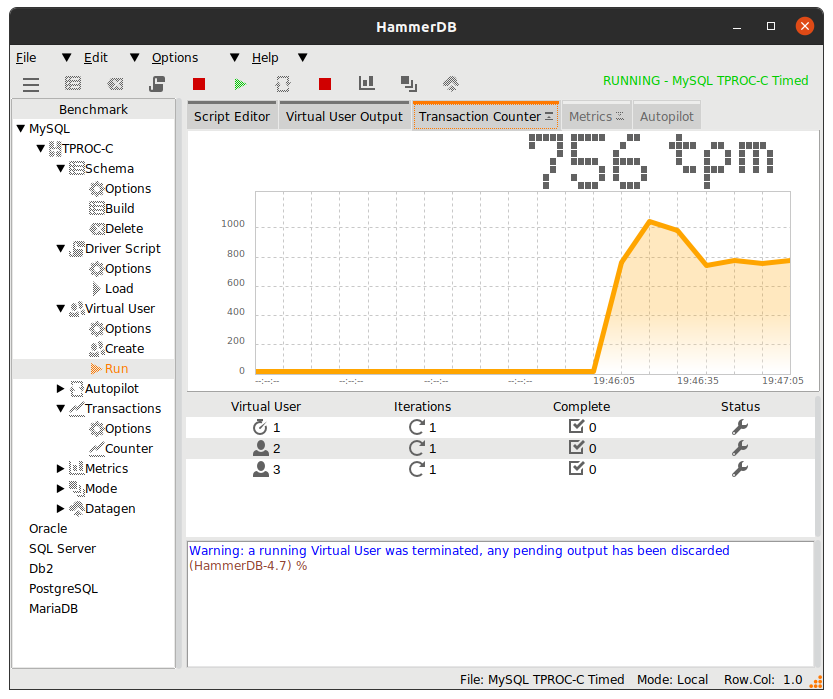
\includegraphics[scale=0.2]{pictures/mysql/vm/tpm1.png}}}
    \quad
    \subfloat{{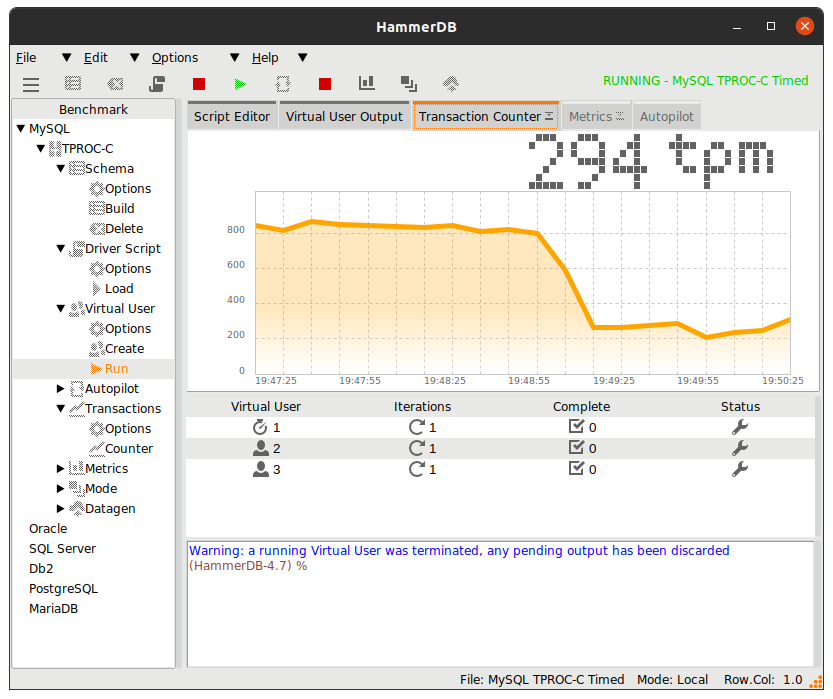
\includegraphics[scale=0.2]{pictures/mysql/vm/tpm2.png}}}
    \quad
    \subfloat{{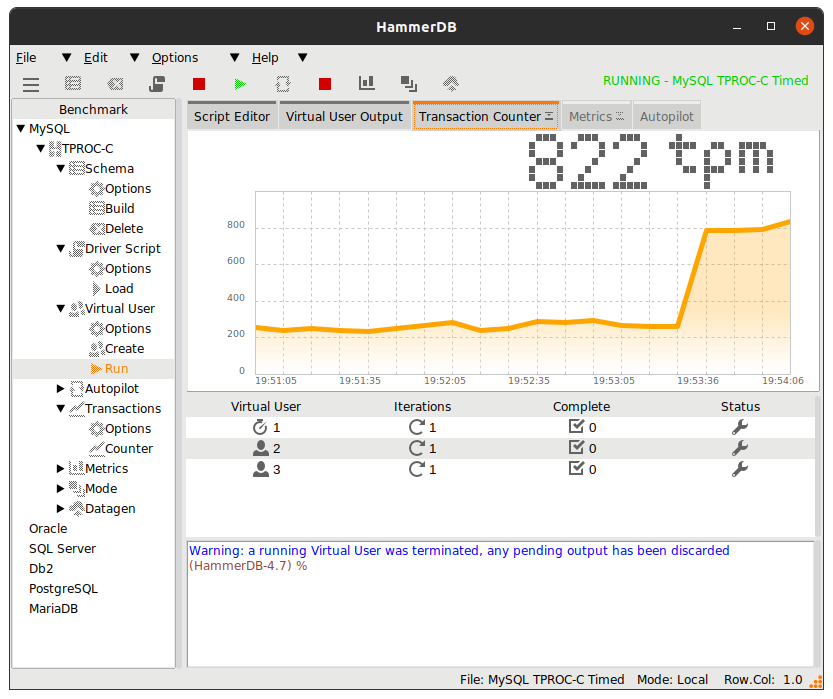
\includegraphics[scale=0.2]{pictures/mysql/vm/tpm3.png}}}
    \quad
    \caption{\lr{TPM} در \lr{VM}}
    \label{fig:mysql:vm:tpm}
\end{figure}
این موضوع ممکن است که به خاطر تحت فشار بیشتر بودن مموری
\lr{VM}
باشد که سریع سعی به خالی کردن
\lr{cache}
مموری دارد و برای اینکه
\lr{cache}
خالی می‌شود سرعت بیشتر می‌شود ولی این موضوع اصلا به نظر من منطقی نیست و احتمالا دلیل دیگری باید وجود داشته
باشد.